\chapter{مقدمه و مفاهیم اولیه}\label{chap:1}
در این فصل به بررسی مفاهیم پایه‌ای و تاریخچه تجزیه اعداد صحیح می‌پردازیم.
\section{تاریخچه و اهمیت تجزیه اعداد}\label{sec:1-1}
اعداد اول همواره به عنوان آجرهای سازنده ریاضیات و پایه و اساس نظریه اعداد شناخته می‌شوند. بر اساس اصول بنیادین ریاضی، هر عدد صحیحِ بزرگتر از یک، یا خود یک عدد اول است و یا می‌توان آن را به صورت ضرب چند عدد اول نوشت. فرایند یافتن این عوامل سازنده، «تجزیه عدد صحیح» \LTRfootnote{Integer Factorization} نامیده می‌شود. در حالی که ضرب کردن دو عدد اولِ بسیار بزرگ به راحتی و در کسری از ثانیه توسط رایانه‌ها انجام می‌شود، فرایند معکوس آن، یعنی یافتن عوامل اولِ یک عدد بسیار بزرگ، مسئله‌ای به شدت زمان‌بر و از نظر محاسباتی پیچیده است. همین عدم تقارن محاسباتی، پایه و اساس سامانه ‌های رمزنگاری کلید عمومی نوین را تشکیل می‌دهد که امروزه امنیت ارتباطات دیجیتال، تراکنش‌های بانکی و تبادل داده‌ها در اینترنت به آن وابسته است.\cite{rivest1978method}
با وجود اینکه اعداد اول نقش محوری در امنیت و محاسبات دارند، نحوه توزیع آن‌ها در میان اعداد طبیعی همواره یکی از اسرارآمیزترین مباحث ریاضیات بوده است. اعداد اول در نگاه اول رفتاری کاملاً تصادفی و بی‌نظم از خود نشان می‌دهند، اما ریاضی‌دانان با استفاده از نمایش‌های هندسی، الگوهای پنهان شگفت‌انگیزی را در میان آن‌ها کشف کرده‌اند. یکی از معروف‌ترینِ این نمایش‌ها «مارپیچ اولام»
 \LTRfootnote{Ulam Spiral}
 است که نشان می‌دهد توزیع اعداد اول کاملاً هم تصادفی نیست.\cite{stein1964visual}
 
 همان‌طور که در 
 \figurename~\ref{pic1}
  مشاهده می‌شود، اگر اعداد طبیعی را به صورت مارپیچی حول یک نقطه مرکزی بنویسیم و اعداد اول را علامت‌گذاری کنیم، الگوهای بصری خاصی نمایان می‌شود. در 
\subfigurename~\ref{subpic1}
 ، نحوه ساختاردهی اولیه این مارپیچ و جایگاه اعداد اول (خانه‌های قرمزرنگ) را در یک مقیاس کوچک نشان می‌دهد. با گسترش این شبکه مارپیچی در مقیاس‌های بسیار بزرگتر، همان‌طور که در 
 \subfigurename~\ref{subpic2}
قابل مشاهده است، اعداد اول به شکل معناداری روی خطوط قطری خاصی متراکم می‌شوند. این رفتار هندسی نشان می‌دهد که مسئله تجزیه اعداد و درک رفتار اعداد اول، فراتر از محاسبات پیچیده جبری، دارای ساختارهای عمیق هندسی و بصری نیز هست که الگوریتم‌های مدرن به دنبال کشف و بهره‌برداری از آن‌ها هستند.
 
\begin{figure}[H]
	\centering
	\begin{subfigure}{0.48\textwidth}
		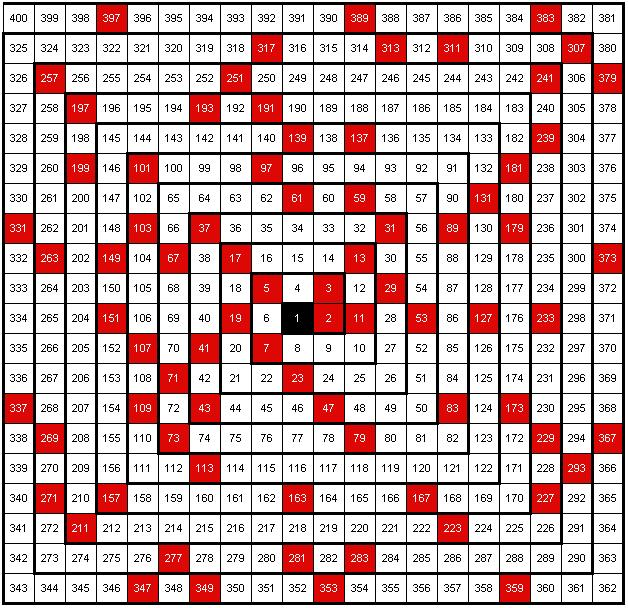
\includegraphics[width=\linewidth, height=7cm]{pic1}
		\caption{ساختار اولیه مارپیچ و جایگاه اعداد اول (خانه‌های قرمزرنگ) در مقیاس کوچک}
		\label{subpic1}
	\end{subfigure}
	\begin{subfigure}{0.48\textwidth}
		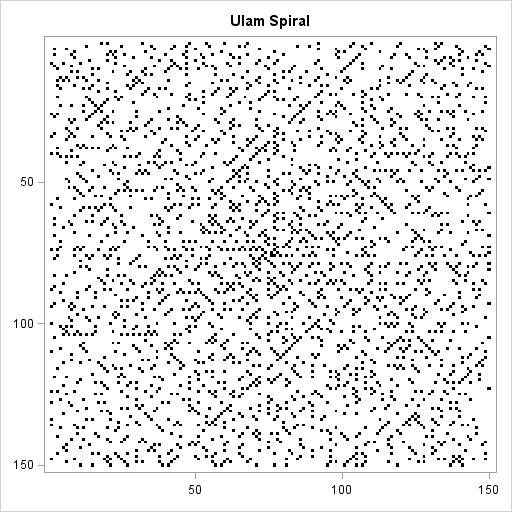
\includegraphics[width=\linewidth, height=7cm]{pic2}
		\caption{ظهور الگوهای قطری و تراکم اعداد اول در مقیاس بزرگتر}\label{subpic2}
	\end{subfigure}
	\caption{نمایش هندسی و الگوهای توزیع اعداد اول در مارپیچ اولام}
	\label{pic1}
\end{figure}

\section{تعاریف پایه ریاضی}\label{sec:1-2}
برای درک بهتر الگوریتم‌های تجزیه، ابتدا باید برخی از مفاهیم اولیه نظریه اعداد را مرور کنیم. قضیه اساسی حساب بیان می‌کند که هر عدد صحیح و بزرگ‌تر از یک مانند $n$ را می‌توان به صورت یکتایی (صرف‌نظر از ترتیب) به صورت حاصل‌ضرب اعداد اول نوشت.\cite{hardy1979introduction} این موضوع در رابطه \eqref{eq1} نشان داده شده است:

\begin{equation}\label{eq1}
	n = p_1^{e_1} \cdot p_2^{e_2} \cdots p_k^{e_k} = \prod_{i=1}^{k} p_i^{e_i}
\end{equation}

که در آن نمادهای $p_i$ اعداد اول متمایز و $e_i$ توان‌های صحیح و مثبت هستند. 

همچنین در بررسی الگوریتم‌ها، گاهی نیاز به تعریف توابع ریاضی برای جداسازی حالت‌های مختلف داریم. برای مثال، تابع نشانگر اول بودن یک عدد مانند $\mathrm{I}(n)$ را می‌توان به صورت یک تابع چندضابطه‌ای به شکل زیر تعریف کرد:

\begin{equation}\label{eq2}
	\mathrm{I}(n) = \begin{cases} 
		1 &  \text{ یک عدد اول باشد} n \text{اگر } \\ 
		0 & \text{در غیر این صورت} 
	\end{cases}
\end{equation}

روابط \eqref{eq1} و \eqref{eq2} پایه و اساس درک الگوریتم‌هایی هستند که در فصل‌های بعدی به آن‌ها خواهیم پرداخت.

\section{ساختار مستند}\label{sec:1-3}

در رَوَندنمای\LTRfootnote{Flowchart}
\figurename~\ref{Flowchart1}
 نمای کلی و سازمان‌دهی مطالب این مستند ارائه می‌شود تا خواننده دید روشنی نسبت به مسیر پیشبرد مباحث داشته باشد:

\begin{figure}[H]
	\centering
	\resizebox{\textwidth}{!}{
		\begin{tikzpicture}[
			node distance=2cm,
			chapbox/.style={draw, rectangle, rounded corners, minimum width=3cm, minimum height=1.2cm, text centered, fill=blue!15, font=\small\bfseries, text width=2.8cm},
			secbox/.style={draw, rectangle, rounded corners, minimum width=3cm, minimum height=1cm, text centered, fill=green!10, font=\footnotesize, text width=2.8cm}, 
			arrow/.style={thick, ->, >=stealth}
			]
			
			\node (chap1) [chapbox] {\hyperref[chap:1]{\rl{فصل ۱: مقدمه}}};
			\node (sec11) [secbox, below of=chap1, yshift=-0.8cm] {\hyperref[sec:1-1]{\rl{۱-۱ تاریخچه و اهمیت تجزیه اعداد اول}}};
			\node (sec12) [secbox, below of=sec11, yshift=-0.5cm] {\hyperref[sec:1-2]{\rl{۱-۲ تعاریف پایه ریاضی}}};
			\node (sec13) [secbox, below of=sec12, yshift=-0.5cm] {\hyperref[sec:1-3]{\rl{۱-۳ ساختار مستند}}};
			
			\node (chap2) [chapbox, left of=chap1, xshift=-1.5cm] {\hyperref[chap:2]{\rl{فصل ۲:\\ مدل سازی ریاضی و الگوریتم ها}}};
			\node (sec21) [secbox, below of=chap2, yshift=-0.8cm] {\hyperref[sec:2-1]{\rl{۲-۱ مقدمه و مدل سازی ریاضی}}};
			\node (sec22) [secbox, below of=sec21, yshift=-0.5cm] {\hyperref[sec:2-2]{\rl{۲-۲ الگوریتم بهینه سازی و روندنما}}};
			
			\node (chap3) [chapbox, left of=chap2, xshift=-1.5cm] {\hyperref[chap:3]{\rl{فصل ۳: توابع زیان و ارزیابی مدل ها}}};
			\node (sec31) [secbox, below of=chap3, yshift=-0.8cm] {\hyperref[sec:3-1]{\rl{۳-۱ مقدمه}}};
			\node (sec32) [secbox, below of=sec31, yshift=-0.5cm] {\hyperref[sec:3-2]{\rl{۳-۲ منظم سازی و رگرسیون ریج}}};
			\node (sec33) [secbox, below of=sec32, yshift=-0.5cm] {\hyperref[sec:3-3]{\rl{۳-۳ تابع زیان هیوبر}}};
			\node (sec34) [secbox, below of=sec33, yshift=-0.5cm] {\hyperref[sec:3-4]{\rl{۳-۴ معادله نرمال}}};
			\node (sec35) [secbox, below of=sec34, yshift=-0.5cm] {\hyperref[sec:3-5]{\rl{۳-۵ الگوریتم های بهینه سازی}}};
			\node (sec36) [secbox, below of=sec35, yshift=-0.5cm] {\hyperref[sec:3-6]{\rl{۳-۶ معیارهای ارزیابی مدل ها}}};
			
			\node (chap4) [chapbox, left of=chap3, xshift=-1.5cm] {\hyperref[chap:4]{\rl{فصل ۴: شبکه‌های عصبی عمیق}}};
			\node (sec41) [secbox, below of=chap4, yshift=-0.8cm] {\hyperref[sec:4-1]{\rl{۴-۱ مقدمه}}};
			\node (sec42) [secbox, below of=sec41, yshift=-0.5cm] {\hyperref[sec:4-2]{\rl{۴-۲ یاخته عصبی مصنوعی}}};
			\node (sec43) [secbox, below of=sec42, yshift=-0.5cm] {\hyperref[sec:4-3]{\rl{۴-۳ شبکه های عصبی چندلایه}}};
			\node (sec44) [secbox, below of=sec43, yshift=-0.5cm] {\hyperref[sec:4-4]{\rl{۴-۴ آموزش شبکه عصبی}}};
			\node (sec45) [secbox, below of=sec44, yshift=-0.5cm] {\hyperref[sec:4-5]{\rl{۴-۵ کاربردهای شبکه های عصبی عمیق}}};
			
			\node (chap5) [chapbox, left of=chap4, xshift=-1.5cm] {\hyperref[chap:5]{\rl{فصل ۵: جمع بندی}}};
			\node (sec51) [secbox, below of=chap5, yshift=-0.8cm] {\hyperref[sec:5-1]{\rl{۵-۱ جمع بندی و نتیجه گیری}}};
			\node (sec52) [secbox, below of=sec51, yshift=-0.5cm] {\hyperref[sec:5-2]{\rl{۵-۲ پیشنهادها برای کارهای آینده}}};
			
			\draw [arrow] (chap1) -- (chap2);
			\draw [arrow] (chap2) -- (chap3);
			\draw [arrow] (chap3) -- (chap4);
			\draw [arrow] (chap4) -- (chap5);
			
			\draw [arrow] (chap1) -- (sec11);
			\draw [arrow] (sec11) -- (sec12);
			\draw [arrow] (sec12) -- (sec13);
			
			\draw [arrow] (chap2) -- (sec21);
			\draw [arrow] (sec21) -- (sec22);
			
			\draw [arrow] (chap3) -- (sec31);
			\draw [arrow] (sec31) -- (sec32);
			\draw [arrow] (sec32) -- (sec33);
			\draw [arrow] (sec33) -- (sec34);
			\draw [arrow] (sec34) -- (sec35);
			\draw [arrow] (sec35) -- (sec36);
			
			\draw [arrow] (chap4) -- (sec41);
			\draw [arrow] (sec41) -- (sec42);
			\draw [arrow] (sec42) -- (sec43);
			\draw [arrow] (sec43) -- (sec44);
			\draw [arrow] (sec44) -- (sec45);
			
			\draw [arrow] (chap5) -- (sec51);
			\draw [arrow] (sec51) -- (sec52);
			
		\end{tikzpicture}
	}
	\caption{گراف ارتباط فصول و ساختار مستند}
	\label{Flowchart1}
\end{figure}
